	% GUIDA VELOCE:
% --------------------------------------------------------------------
% X INIZIA UN UNOVO CAPITOLO:
% \chapter{??? NOME CAPITOLO}}
% \section{ ?? }
% \subsection{ ?? }
%
% --------------------------------------------------------------------
% PAROLA CONTENUTA NEL GLOSSARIO:
% scrivere la parola seguita da $^g$
% esempio: User$^g$
%
% --------------------------------------------------------------------
% PER ANDARE A CAPO SENZA RIENTRO INSERIRE:
% \\
%
% --------------------------------------------------------------------
% GRASSETO:
% \textbf{parola}
%
% --------------------------------------------------------------------
% CORSIVO:
% \emph{parola}
% --------------------------------------------------------------------
% PER SCRIVERE IN ROSSO:
% \red{parola}
%
% --------------------------------------------------------------------
% PER SCRIVERE TRA VIRGOLETTE
% ''parola''
%
% --------------------------------------------------------------------
% PER EVITARE IL RIENTRO AUTOMATICO DI UN CAPOVERSO:
% \noindent testo....
%
% --------------------------------------------------------------------

% PER SCRIVERE CARATTERI PARTICOLARI COME: { } _ ecc.. SCRIVERLI PRECEDUTI DA \
% ES: \{ \_
%
% --------------------------------------------------------------------
% X INSERIRE UN LINK:
% \url{http://www.math.unipd.it/~tullio/IS-1/2011/Progetto/C3.pdf}
%
% --------------------------------------------------------------------
% PER COMMENTARE INTERE PARTI:
% \comment{ comment }
%
% --------------------------------------------------------------------
% PER SCRIVERE NOTE DURANTE IL TESTO:
% parola \footnote{ note riguardanti la parola }
%
% --------------------------------------------------------------------
% PER SCRIVERE CODICE SORGENTE:
%
% \lstset{language=c++,
% stringstyle=\color{blue}\textrm,
% commentstyle=\rmfamily, numbers= none}

% \begin{lstlisting}
% CODICE
% \end{lstlisting}
%
% --------------------------------------------------------------------
% !!!!!!!! PER COSE + COMPLESSE VEDI: !!!!!!!!!!!!!!!!!!!!!!!
% !!!!!!!! PMAC/latex/GUIDA LATEX!!!.tex !!!!!!!!!!!!!!!!!!!!!!!

% per tutto il resto chiedi a lory prima di fare/scrivere cazzate !!!!!!!!!!



\documentclass[10pt,a4paper]{article}

\usepackage[italian]{babel}
\usepackage[T1]{fontenc}
\usepackage[utf8x]{inputenc} % uso utf8x xk x linux, mentre latin1 è per windows
\usepackage{lmodern} %insieme di font molto completo consigliato da LatexFacile pg13 in basso
\usepackage{microtype} %migliora riempimento delle righe. vedi LatexImpaziente pg41
%attiva il rientro di ogni prima riga di ogni sezione: capitolo,paragrafo ecc. vd LatexImpaziente pg41
\usepackage{indentfirst}
\usepackage{graphicx} % per inseire immagini
\usepackage[usenames,dvipsnames]{color}
\usepackage{lastpage} %serve per poter scrivere page 1 of N
% setta i bordi della pagina: dx e sx 3.2cm di rientro + nel lato di rilagatura rientra di altri 0mm
\usepackage[a4paper,top=3cm,bottom=3cm,left=3.2cm,right=3.2cm, bindingoffset=0mm]{geometry}
\usepackage{listings} % per inserire codice sorgente
\usepackage{float} % per gestire oggetti flottanti ( es immagini tabelle posizionebili con "H" che forza il posizionamento nel punto specifico )

% serve per creare tabelle lunghe + di una pagina con \begin{longtable} (vd Tabelle.pdf pg11-12)
\usepackage{longtable}

\usepackage{fancyhdr} % per impostare lo stile della pagina più personalizzato, + fancyhdr ( per regolare testatina e piè di pagina ) vedi itfancyhrd

%per \EUR
\usepackage{marvosym}

\pagestyle{fancy}
% settaggi di pagestyle(fancy)
\lhead{
\includegraphics[scale=0.20]{images/SevenFold_small}}
%\chead{}
\rhead{\textbf{{%
\NomeDocumento - \VersioneAttuale \\ Data versione attuale: \DataRilascio \\ e-mail: \mail{sevenfold@palomino.it}}}}
\lfoot{\NomeDocumento}
\cfoot{}
\rfoot{ \textbf \thepage\ di \pageref{LastPage}}
\renewcommand{\footrulewidth}{0.4pt}

%ridefinisco il plain per cosare l'indice (a questo punto si potrebbe lasciare tutto il documento in plain
\fancypagestyle{plain}{
\lhead{
\includegraphics[scale=0.20]{images/SevenFold_small}}
%\chead{}
\rhead{\textbf{{%
\NomeDocumento - \VersioneAttuale \\ Data versione attuale: \DataRilascio \\ e-mail: \mail{sevenfold@palomino.it}}}}
\lfoot{\NomeDocumento}
\cfoot{}
\rfoot{ \textbf \thepage\ di \pageref{LastPage}}
\renewcommand{\footrulewidth}{0.4pt}
}

% da ultimo:
\usepackage{hyperref} %x l'interpretazione di indirizzi o link ipertestuali (vd LatexImpaziente pg47 )
\hypersetup{backref, colorlinks=true, linkcolor=black, urlcolor=black}

\usepackage{url} % x l'interpretazioni di internet o link ipertestuali (vd LatexImpaziente pg47 )
%\UrlFont{color =blue}
%\urlstyle{helvetic}

% Define a new 'leo' style for the package that will use a smaller font.
\makeatletter
\def\url@leostyle{%
  \@ifundefined{selectfont}{\def\UrlFont{\sf}}{\def\UrlFont{\small\ttfamily}}}
\makeatother
%% Now actually use the newly defined style.
\urlstyle{leo}


\newcommand{\mail}[1]{\textcolor{Black}{ \texttt{#1}}} %per interpretare mail (vd LatexImpaziente pg47 )
\newcommand{\cambiaFont}[2]{{\fontencoding{T1}\fontfamily{#1}\selectfont#2}}
\newcommand{\red}[1]{ \textcolor{red}{#1} } % per scrivere testo in rosso
\newcommand{\comment}[1]{} % per inserire commenti

\newcommand{\attribute}[2]{ \item[\textcolor{PineGreen}{ \texttt{#1}}] \textcolor{PineGreen}{\texttt{#2\\}}\ \ \ }
\newcommand{\method}[2]{ \item[\textcolor{MidnightBlue}{ \texttt{#1}}] \textcolor{MidnightBlue}{ \texttt{#2\\}}\ \ \ }

\newcommand{ \class}[1]{ \item[-] \texttt{#1} }
\newcommand{\virgolette}[1]{``{#1}''}



% INSERIRE QUI IL NOME DEL DOCUMENTO SEGUITO DA UNO SPAZIO
% ( così il nome si imposta in automatico nelle varie ricorrenze standard)
\newcommand{\NomeDocumento}{Scrivi in questo documento k poi uniamo tutto }

% INSERIRE QUI LA DATA DEL RILASCIO DELLA VERSIONE ATTUALE
\newcommand{\DataRilascio}{2012/04/02}

% INSERIRE LA VERSIONE ATTUALE
\newcommand{\VersioneAttuale}{v2.0.0}

% INSERIRE QUI L'ACRONIMO DEL DOCUMENTO. ESEMPIO: Analisi Dei Requisiti = AR
% Quando inserite l'acronimo qui, dovete rinominare i file presenti nella cartella
% del tipo '??-cap1-NomeCapitolo.tex' sostituendo i '??' con l'acronimo scelto!!
\newcommand{\AcronimoDocumento}{DP}

\begin{document}


% --------------------------------------------------------------------

% TITOLO ( 1° pagina)

\vspace*{2.5cm}
\begin{center}

%\cambiaFont{Cyklop}{Sevenfold}
%\cambiaFont{fve}{\Huge{Sevenfold}}

\includegraphics[scale=0.35]{images/SevenFold_big}

\vspace{2cm}

\cambiaFont{fve}{\Huge{\NomeDocumento}}\\
\vspace*{1cm}

è richiesto: circa 15 pagine a testa..

\end{center}


% --------------------------------------------------------------------

% INFORMAZIONI DEL DOCUMENTO ( 1° pagina)

\vspace*{2cm}




% --------------------------------------------------------------------

% SOMMARIO ( 2° pagina)

\newpage

\vspace*{0.5cm} % il vertical space va preceduto da una riga vuota!!!
\begin{center}

\textbf{{\huge{Sommario}}}

Questo documento contiene la struttura del sistema Woty, analizzando nel dettaglio i suoi componenti.

\vspace*{0.2cm} % il vertical space va preceduto da una riga vuota!!!

\end{center}


% --------------------------------------------------------------------



% --------------------------------------------------------------------
% INDICI:

\newpage

% INDICE CAPITOLI
\tableofcontents % genera l'indice di tutto il documento

\let\cleardoublepage\clearpage % toglie la pagina bianca dopo l'indice

% INDICE TABELLE
\listoftables

% INDICE FIGURE
\listoffigures


% --------------------------------------------------------------------

% INTRODUZIONE ( 1° CAPITOLO ) QUESTO CAPITOLO VA MESSO IN OGNI DOCUMENTO!!!!!!!!

\newpage
\section{Pianificazione del lavoro}

\subsection{Introduzione}
Il gruppo di lavoro si trova ad aver progettato e in amplia parte sviluppato il software in questione nell'ambito del progetto del corso di studi Ingegneria del software. \\Per poter procedere ad una fase successiva il team si prefigge l'obiettivo di effettuare una analisi di mercato e un relativo studio di fattibilità per ottenere il via libera per la realizzazione di un prodotto funzionante e la sua commercializzazione.\\In questo documento intendiamo quindi presentare l'elaborato della \virgolette{seconda fase} (vedi capitolo seguente) per riuscire poi a proseguire nella realizzazione del progetto, vediamo in dettaglio la suddivisione del lavoro e lo stato di avanzamento:

\subsection{Fasi di avanzamento}

\vspace*{0.5cm}

\begin{figure}[H]
\centering
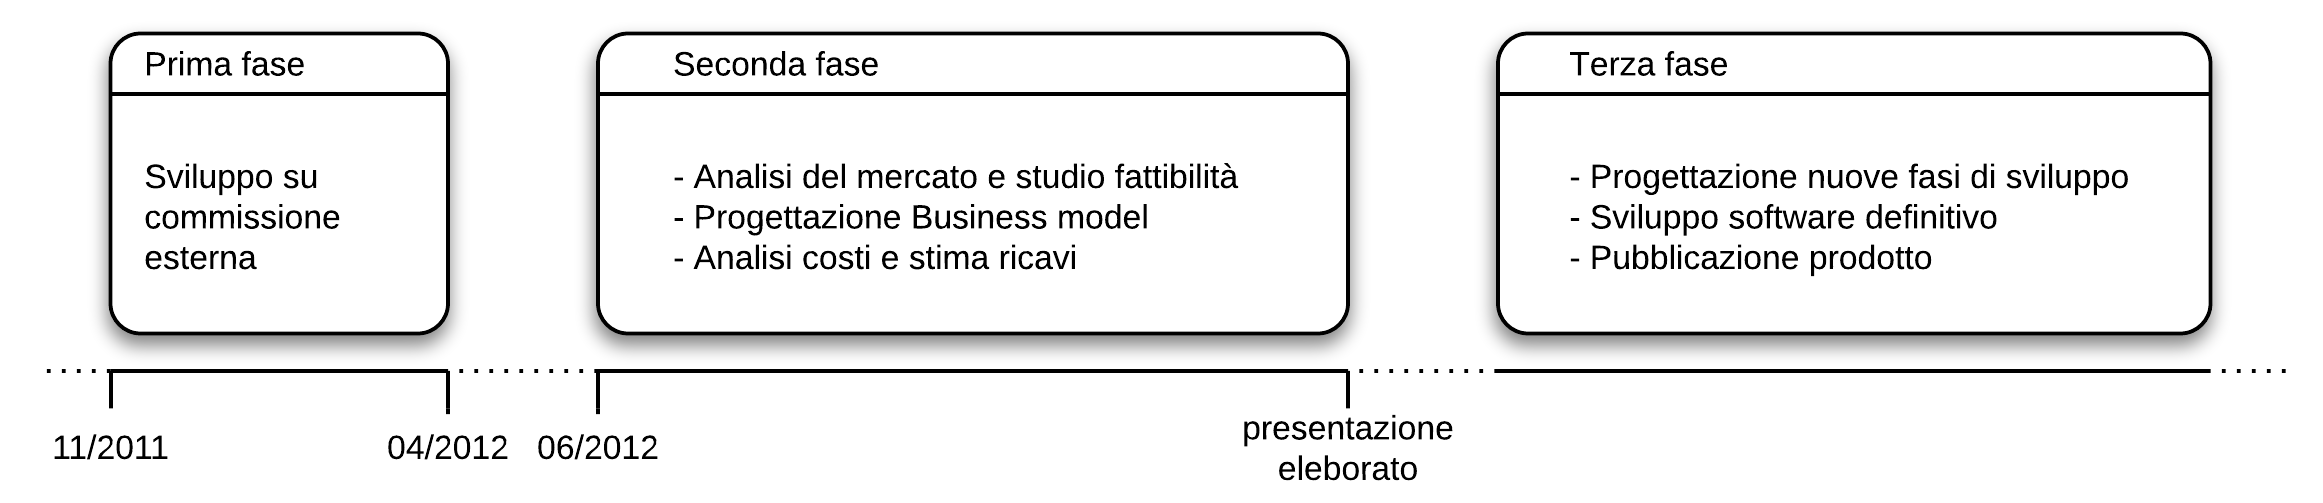
\includegraphics[scale=0.7]{images/avanzamento.png}
\caption{Avanzamento lavoro}
\end{figure} 

\vspace*{0.5cm}

In figura \virgolette{Avanzamento lavoro} si può vedere l'avanzamento temporale del progetto e la suddivisione in fasi del lavoro del nostro gruppo. È da sottolineare ancora una volta che il presente documento intende presentare i risultati della fase due per proporre l'avanzamento del progetto alla sua fase conclusiva. Vediamo formalmente la divisione in fasi: \\

\begin{itemize}
\item Prima fase (corso Ingegneria del software):
\begin{itemize}
\item Sviluppo su commissione esterna 
\end{itemize}
\end{itemize}

\begin{itemize}
\item Seconda fase (presentata in questo documento):
\begin{itemize}
\item Analisi del mercato e studio fattibilità
\item Progettazione Business model
\item Analisi costi e stima ricavi
\end{itemize}
\end{itemize}

\begin{itemize}
\item Terza fase (all'approvazione della fase due):
\begin{itemize}
\item Progettazione nuove fasi di sviluppo
\item Sviluppo software definitivo
\item Pubblicazione prodotto
\end{itemize}
\end{itemize}

\newpage

\subsection{Fase due: strumenti e risorse}
Per affrontare con massima efficienza la fase due del progetto il nostro team di lavoro deve avvalersi di alcune risorse, sia intese come strumenti per facilitare il lavoro, sia come conoscenze che i componenti del gruppo hanno già in parte apprese dal corso di Sviluppo e Gestione dei Progetti e devono mettere in pratica. In questo capitolo vediamo come si intende affrontare questa fase, quali strumenti intendiamo utilizzare per garantire un alta qualità del lavoro e quali figure ci sono indispensabili per raggiungere un livello di dettaglio adeguato.

\subsubsection{Strumenti}
\begin{itemize}
\item Git: software per il versionamento del documenti, essenziale al nostro team per poter lavorare liberamente su documenti senza rischiare di perdere avanzamenti importanti svolti da altri componenti del gruppo.
\item Teamspeak: software per la comunicazione vocale tramite la rete internet che ci permette di compiere meno movimenti sul territorio e poter svolgere comunque il nostro lavoro. Tuttavia non sarà uno strumento sufficiente per eliminare gli incontri settimanali organizzati dal gruppo per aggiornare lo svolgimento e discutere gli eventuali problemi riscontrati.
\item Google Drive: utility offerta da google per la condivisione di documenti sui quali lavorare in modo concorrente e in tempo reale.
\item Editor LaTex: software che permette la stesura di documenti in modo formale e pulito. Verrà utilizzato per la scrittura e l'impaginazione di tutti i documenti ufficiali in questo progetto.
\end{itemize}

\subsubsection{Figure}
In figura \virgolette{Organization Breakdown Structure} è mostrata l'organizzazione adottata dal team per ottenere una migliore gestione carico di lavoro. È essenzialmente un organizzazione a matrice debole, che vede il Capo progetto come Project Manager e Come Manager di Funzione i vari esperti e capi. Vediamo ora lo schema e la descrizione di ogni ruolo:

\vspace*{0.5cm}

\begin{figure}[H]
\centering
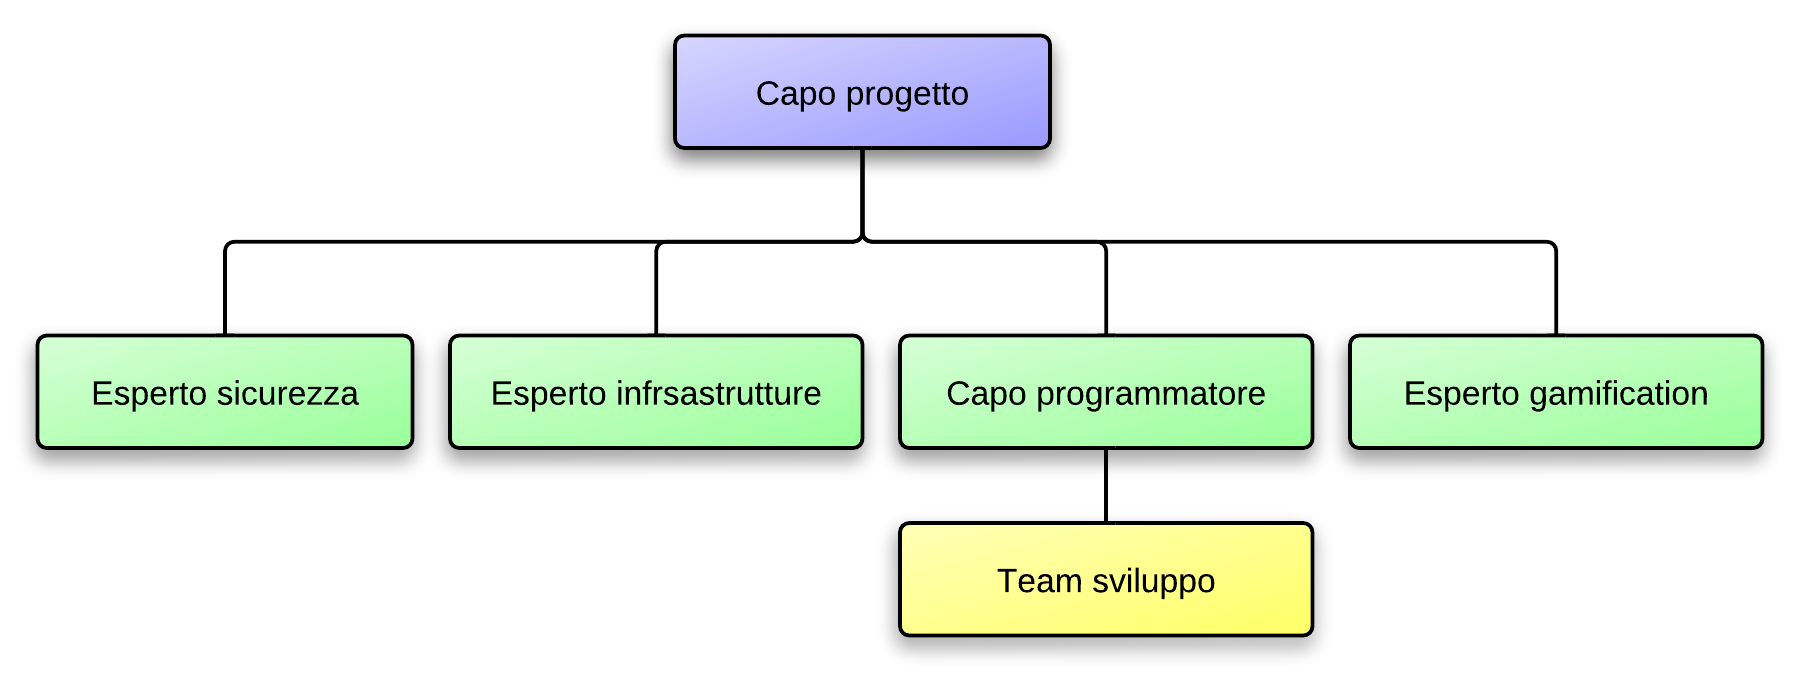
\includegraphics[scale=1]{images/obs.png}
\caption{Organization Breakdown Structure}
\end{figure}

\vspace*{0.5cm}

\begin{itemize}
\item Capo progetto: ha il compito che amministrare e gestire tutti team di lavoro, controllare le tempistiche e la qualità del loro lavoro. Dovrà interagire con il responsabile di ogni gruppo di lavoro per tenersi sempre aggiornato sull'avanzamento, è anche responsabile di eventuali richiami in caso qualche team non stia lavorando secondo gli accordi.
\item Esperto sicurezza: persona che avendo esperienza nel settore della sicurezza può rispondere alle questioni che vengono sollevate durante lo studio di fattibilità riguardante la realtà di applicazione del nostro software. Può indicare con precisioni quali sono le difficoltà che potremo riscontrare nell'offrire il nostro software ad una società e può dare informazioni attendibili riguardo i dettagli tecnici del settore. 
\item Esperto infrastrutture informatiche: figura che conoscendo adeguatamente le infrastrutture, la loro gestione e manutenzione può aiutare a quantificare gli investimenti necessari sia da parte degli sviluppatori che da parte degli acquirenti. Deve confrontarsi con l'esperto in sicurezza per capire le esigenze del settore d'applicazione del software.
\item Capo programmatore: persona con il compito di programmare la restante parte del software. Ha il compito di fornire stime sulle tempistiche di sviluppo e di testing sul software generato. È formalmente a capo del team di sviluppo del software.
\item Esperto gamification: esperto che grazie alle sue conoscenze saprà valutare allo stato attuale come implementare al meglio la gamification e a che livello le persone sono disposte ed affrontarla nell'ambito della sicurezza sul lavoro.
\end{itemize}

\subsubsection{Responsabilità}
Da sottolineare il fatto che queste figure possono essere ricoperte da più persone sia contemporaneamente che in momenti diversi, e di tutto il loro lavoro sarà tenuta traccia sotto forma di documentazione.
Le responsabilità che ogni figura ha sull'elaborato sono mostrate in figura \virgolette{Responsabilità} e indicano il peso delle decisioni di ogni figura sul lavoro che sta supervisionando o svolgendo:

\vspace*{0.5cm}

\begin{figure}[H]
\centering
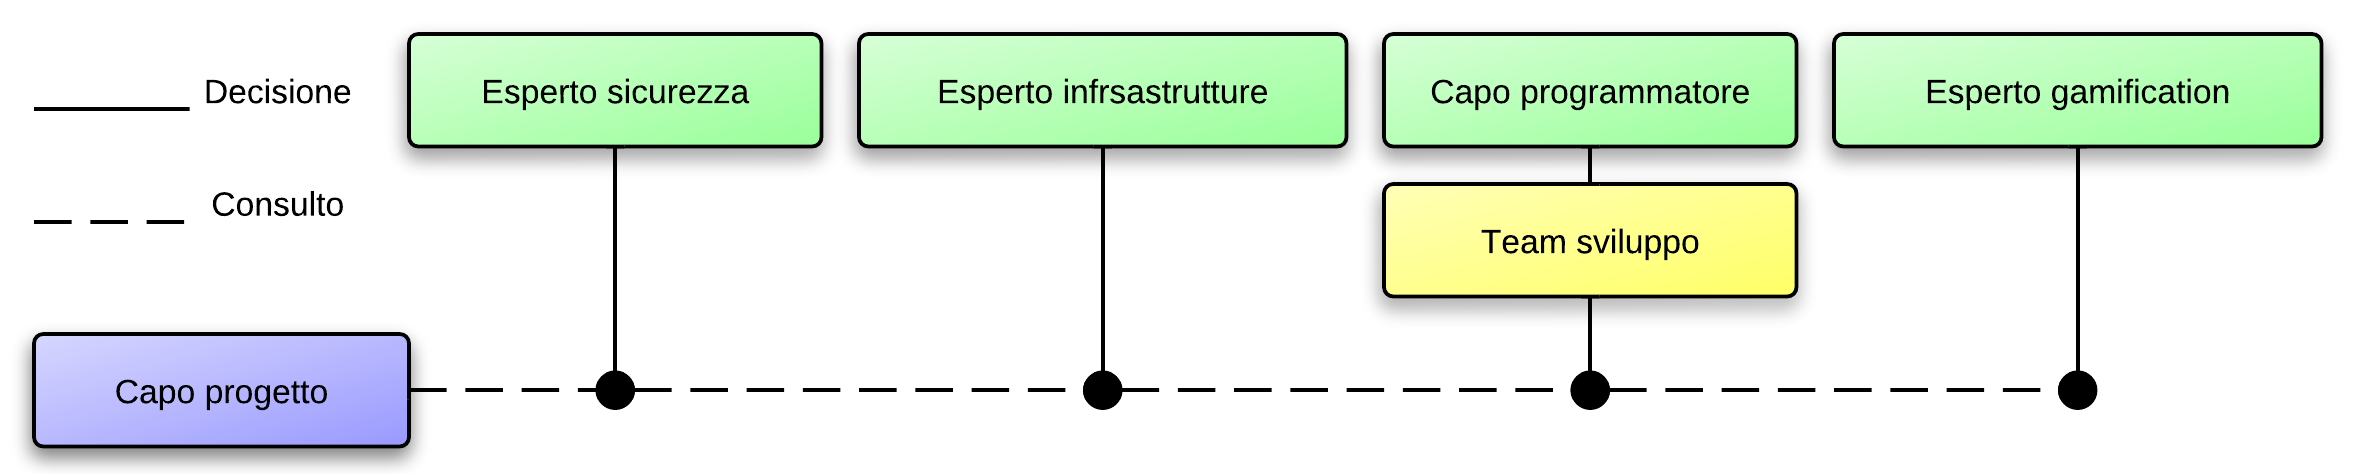
\includegraphics[scale=0.8]{images/resp.png}
\caption{Responsabilità}
\end{figure}

\vspace*{0.5cm}

Possiamo vedere nel diagramma \virgolette{Responsabilità} come il capo progetto abbia potere di consulenza e supervisione su tutte le parti del gruppo di lavoro, ma che l'aspetto decisionale spetti direttamente al responsabile di quella attività.

\newpage

\subsection{Pianificazione temporale}

Il nostro team per garantire un adeguata qualità del lavoro si impegna a seguire uno schema temporale che ricopre tutto lo svolgimento della fase due del progetto, quindi ogni figura deve svolgere delle attività prestabilite seguendo un calendario preciso. \\Eventuali discrepanze con le tempistiche da parte di uno qualsiasi dei membri del gruppo può e deve essere affrontata sotto la diretta supervisione del capo progetto, che di volta in volta dovrà decidere come precedere per risolvere il problema. \\Vediamo ora in figura \virgolette{Gantt} la schedulazione prevista:

\vspace*{0.5cm}

\begin{figure}[H]
\centering
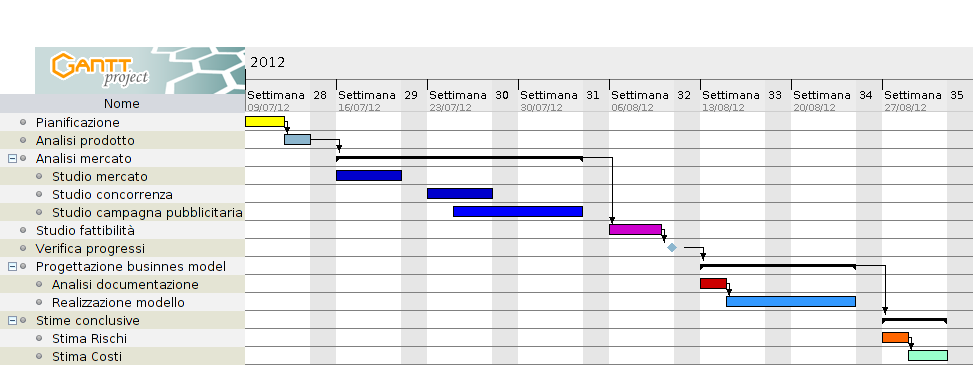
\includegraphics[scale=0.4]{images/Gantt.png}
\caption{Gantt}
\end{figure}

\vspace*{0.5cm}

Dato il grado non troppo elevato di questa fase dovuta ad una progettazione strutturata su molte figure diverse e specializzate, si è ritenuto opportuno lo sviluppo del progetto seguendo un ciclo di vita cosiddetto a cascata, che prevede quindi il susseguirsi delle varie fasi auto-conclusive, e che alla loro chiusura prevedono la documentazione necessaria e sufficiente per l'avanzamento alla fase successiva.

\subsubsection{Descrizione delle fasi}
\begin{itemize}
\item Analisi di mercato: è la prima fase nello sviluppo del progetto. È dedicata ad un analisi a livello di mercato per ottenete le informazioni necessarie ad uno sviluppo del prodotto mirato nella fascia di mercato corretta, e con una eccellente grado di soddisfazione del cliente.
\begin{itemize}
\item Raccolta dati sicurezza: fase dedicata all'ispezione del mercato sotto l'aspetto della sicurezza, per valutare come sia attualmente sviluppato la fascia di mercato dove il nostro prodotto andrà collocarsi.
\item Relazione sicurezza: organizzazione e stesura dei dati raccolti riguarda la sicurezza nella fase precedente.
\item Raccolta dati gamification: fase debita a verificare come il concetto della gamification sia radicato nella fascia di mercato che vogliamo ricoprire, alla fine di questa fase si deve essere in grado di valutare la conoscenza da parte del cliente di questo concetto e la sua capacità di assimilarlo.
\item Relazione gamification: organizzazione e stesura dei dati raccolti riguardo la gamification nella fase precedente.
\end{itemize}
\item Studio fattibilità: è la seconda fase del progetto e ha lo scopo di valutare ed analizzare tutti i dati raccolti nella fase di analisi di mercato. È mirata a decidere se e come il nostro prodotto possa possa domanire sugli eventuali competitor.
\begin{itemize}
\item Realtà sicurezza: analisi dei dati raccolti riguardo la sicurezza.
\item Software: studio di fattibilità elaborato del capo programmatore con lo scopo di fare uno studio di fattibilità riguardante allla parte software che deve essere ancora sviluppata.
\item Realtà gamification: analisi dei dati raccolti riguardo la sicurezza.
\item Infrastrutture: studio di fattibilità con lo scopo di determinare quali infrastrutture siano necessarie, come organizzarle e gestirle per una performance eccellente.
\end{itemize}
\item Verifica progressi: fase di verifica dell'avanzamento del lavoro, dove il capo progetto deve assicurarsi che i lavori siano arrivati al punto prestabilito. Si riportano eventuali problemi riscontrati e necessità. Qui deve essere finita la fase di raccolta dati e analisi per iniziare con la creazione del Business Model. 
\item Progettazione Business Model:
\begin{itemize}
\item Analisi dati mercato: si analizzano i dati risultanti dalla fase di analisi di mercato per ottenere una chiara idea per ideare un ottimo business model.
\item Analisi dati fattibilità: si analizzano i dati risultanti dallo studio di fattibilità e si decide come il business model dovrà essere orientato.
\item Realizzazione modello: fase di progettazione del business model.
\end{itemize}
\item Stima rischi: fase dedicata alla stima di successo o insuccesso del prodotto, si decide come affrontare eventuali problemi o ritardi nello sviluppo.
\item Stima costi: si effettua una previsione in base ai dati elaborati fino ad ora per lo sviluppo del software rimanente e del successivo inserimento nel mercato.
\end{itemize}

\newpage
\subsubsection{Distribuzione delle risorse}
Alcuni compiti saranno svolti dal membro del gruppo che ricopre il ruolo corrispondente, ad esempio il compito \virgolette{Raccolta dati sicurezza} sarà svolto dal membro del gruppo che ricopre la figura di \virgolette{Esperto sicurezza}, altri saranno svolti da più membri contemporaneamente, come ad esempio \virgolette{Progettazione Business Model}, ma vediamo in dettaglio la distribuzione delle risorse del team rispetto le fasi operative: \\

\begin{figure}[H]
\centering
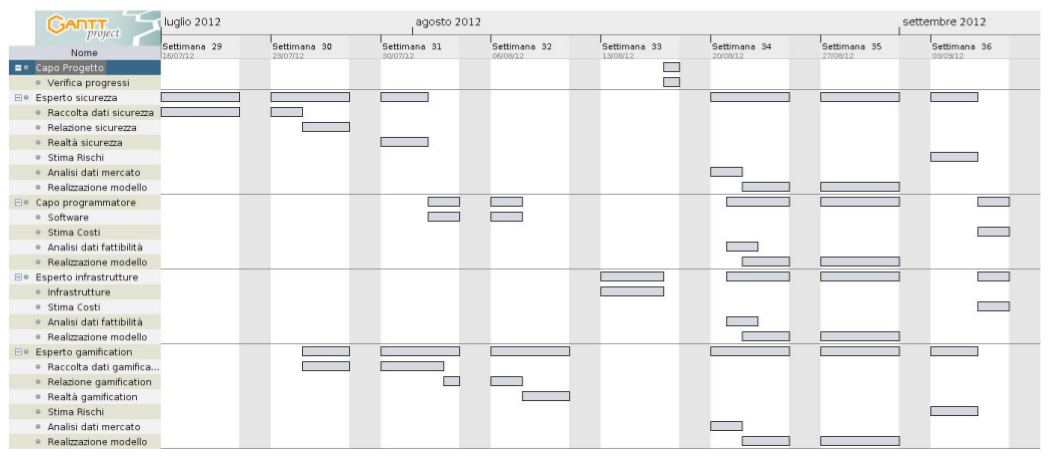
\includegraphics[scale=0.8]{images/risorse.png}
\caption{Distribuzione risorse}
\end{figure}

\vspace*{0.5cm}

Nella figura \virgolette{Distribuzione risorse} si può vedere come le varie figure partecipanti al lavoro siano impegnate temporalmente su tutto il periodo di attività.

\subsubsection{Pianificazione oraria e dei costi}

In questa sezione sarà proposto il preventivo che risulta dalle ipotesi sulla quantità di ore che servirà ad ogni figura professionale per svolgere la propria parte di progetto.\\
Il preventivo sarà calcolato tramite i costi medi orari (CMO) riassunti nella seguente tabella:\\

\begin{longtable}{ | p{5cm} | p{3.4cm} |}
\caption{Compenso orario delle figure professionali}\\
\hline
\endfirsthead
\multicolumn{2}{r}{\textit{(Continua alla pagina successiva)}}
\endfoot
\multicolumn{2}{l}{\textit{(Continua dalla pagina precedente)}}
\endhead
\hline
\endlastfoot
\textbf{Figura professionale} \ & \textbf{CMO}\\
\hline
\rule[-2mm]{0mm}{0.7cm}
Capo progetto & \EUR \ 40 \\
\hline
\rule[-2mm]{0mm}{0.7cm}
Esperto mercato & \EUR \ 25 \\
\hline
\rule[-2mm]{0mm}{0.7cm}
Esperto marketing & \EUR \ 25 \\
\hline
\rule[-2mm]{0mm}{0.7cm}
Tecnico informatico & \EUR \ 30 \\
\hline
\end{longtable}


\begin{longtable}{ | p{6cm} | p{3.5cm} | p{3.5cm} |}
\caption{Preventivo costi totali per ogni figura professionale}\\
\hline
\endfirsthead
\multicolumn{3}{r}{\textit{(Continua alla pagina successiva)}}
\endfoot
\multicolumn{3}{l}{\textit{(Continua dalla pagina precedente)}}
\endhead
\hline
\endlastfoot
\textbf{Figura professionale} \ & \textbf{Ore preventivate} \ & \textbf{Costi preventivati} \\
\hline
\rule[-2mm]{0mm}{0.7cm}
Capo progetto & 96 (32 giorni) & \EUR \ 3.840\\
\hline
\rule[-2mm]{0mm}{0.7cm}
Esperto sicurezza & 130 (26 giorni)& \EUR \ 3.640 \\
\hline
\rule[-2mm]{0mm}{0.7cm}
Esperto infrastrutture informatiche & 75 (15 giorni) & \EUR \ 1.875 \\
\hline
\rule[-2mm]{0mm}{0.7cm}
Capo programmatore & 90 (15 giorni) & \EUR \ 2.700 \\
\hline
\rule[-2mm]{0mm}{0.7cm}
\textbf{Totale} & \textbf{495 (9 settimane)} & \textbf{\EUR \ 14.655} \\
\hline
\end{longtable}

Viene inoltre proposta la tabella con i costi preventivati per ogni fase di progetto indicata nella pianificazione:

\begin{longtable}{ | p{6cm} | p{4.4cm} |}
\caption{Preventivo costi per fase di progetto}\\
\hline
\endfirsthead
\multicolumn{2}{r}{\textit{(Continua alla pagina successiva)}}
\endfoot
\multicolumn{2}{l}{\textit{(Continua dalla pagina precedente)}}
\endhead
\hline
\endlastfoot
\textbf{Fase di progetto} \ & \textbf{Costi preventivati}\\
\hline
\rule[-2mm]{0mm}{0.7cm}
Analisi e pianificazione iniziale & \EUR \ 1.000 \\
\hline
\rule[-2mm]{0mm}{0.7cm}
Analisi di mercato & \EUR \ 3.040 \\
\hline
\rule[-2mm]{0mm}{0.7cm}
Studio di fattibilità & \EUR \ 2.580 \\
\hline
\rule[-2mm]{0mm}{0.7cm}
Progettazione business model & \EUR \ 5.785 \\
\hline
\rule[-2mm]{0mm}{0.7cm}
Stima rischi/Stima costi & \EUR \ 2.250 \\
\hline
\rule[-2mm]{0mm}{0.7cm}
\textbf{Totale} & \textbf{\EUR \ 14.655} \\
\hline
\end{longtable}

Questi dati saranno poi confrontabili con il quantitativo orario svolto effettivamente e le spese sostenute nel consuntivo.

\end{document}